\begin{figure}[h!]
	\centering
	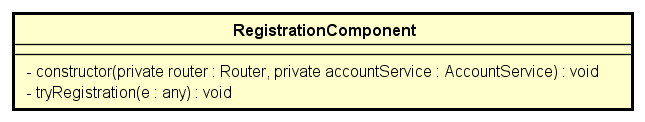
\includegraphics[scale=0.8]{res/sections/SpecificaFrontEnd/Components/Disegnetti/registration.png}
	\caption{Diagramma della classe RegistrationComponent}
\end{figure}

\begin{itemize}
    \item \textbf{Descrizione:}\\
    È il componente che descrive la pagina di registrazione dell’applicazione, mette a disposizione dell’utente un form dove iserire le informazioni necessarie alla creazione di un nuovo account utente. Gestisce le operazioni e la logica applicativa per la registrazione.
    \item \textbf{Utilizzo:}\\
    Questo componente viene istanziato dinamicamente dal servizio Router del framework Angular quando viene richiesta la pagina di registrazione.
	\item \textbf{Metodi:}
    \begin{itemize}
    	\item \emph{-constructor(private router: Router, private accountService: AccountService)}\\
    	Crea un istanziazione di RegistrationComponent\\
    	\textbf{Parametri:}
    		\begin{itemize}
    			\item \emph{-router: Router}
    			Necessario per l'importaziine del Router
    			\item \emph{-accountService: AccountService}
    			Necessario per l'importazione di AccountService
    		\end{itemize}
    	\item \emph{-tryRegistration(e: any)}\\
    	Tenta di registrare un utente\\
    	\textbf{Parametri:}
    		\begin{itemize}
    			\item \emph{+e: any}\\
    			Contiente i dati dell'utente da registrare
    		\end{itemize}
    \end{itemize}
\end{itemize}